
\chapter{Проектирование ОЭП}
\newthought{Проектирование}\marginnote{\allcaps{ПРОЕКТИРОВАНИЕ}}~--- разработка проектной, конструкторской и другой технической документации, предназначенной для создания новых видов и образцов продукции промышленности.

\noindent
\textsc{Цель проектирования}\marginnote{\allcaps{ЦЕЛЬ ПРОЕКТИРОВАНИЯ}}~--- разработка нового изделия.

В процессе проектирования происходит поиск вариантов создания оптико-электронных приборов, его возможных конструкций, разработка и уточнение схем, теоретическое и экспериментальное исследование характеристик предполагаемых инженерных решений.

\noindent
\textsc{Конструирование}\marginnote{\allcaps{КОНСТРУИРОВАНИЕ}} является составной частью проектирования и заключается в разработке конкретного варианта изделия на основе проведенных предварительных исследований. При этом создается конструкция проектируемого изделия: устройство, состав, взаимное расположение частей и элементов, способ их соединения и взаимодействия с учетом используемых материалов, технологии изготовления.

В процессе проектирования выпускают чертежи сборочных единиц и деталей, схемы, рассчитывают допуски на погрешности и технологию изготовления и сборки деталей, устанавливают технические условия на прибор, составляют техническое описание, разрабатывают другую конструкторскую документацию, необходимую для изготовления и эксплуатации изделия.

\section{Уровни проектирования}
Разработка сложных систем, какими являются ОЭП, проводится в определенной последовательности.

Отправной точкой создания любой системы являются выбор и формулировка цели проектирования. Необходимость создания нового изделия определяется как развитием конкретного направления техники, так и запросами потребителей (научных и производственных учреждений, человека-оператора). 

Обоснование исходных данных требует учета назначения системы, основных видов ее взаимодействия с другими системами или подсистемами, если она является подсистемой, входящей в состав другой более крупной системы, влияния внешних факторов.

В результате указанного рассмотрения должна быть получена полная совокупность исходных данных для проектирования прибора. 

Результатом проделанной работы является техническое задание~(ТЗ) на прибор, после утверждения которого можно переходить к собственно проектированию.

Различают следующие основные уровни проектирования:
\begin{itemize}
	\item информационно-логический;
	\item системотехнический;
	\item схемотехнический;
	\item конструкторский;
	\item технологический.
\end{itemize}

Первые три уровня иногда объединяют в единый функциональный, или схемный уровень проектирования.

В\marginnote{\allcaps{ИНФОРМАЦИОННО-ЛОГИЧЕСКИЙ УРОВЕНЬ}} процессе проектирования на информационно-логическом уровне определяется конкретная структура данного прибора, определяются связи функциональных устройств между собой и устанавливаются требования технических заданий на проектирование отдельных функциональных устройств, исходя из требований ТЗ на прибор в целом. ТЗ на проектирование того или иного устройства содержит требования к сигналам, информации и командам, вырабатываемым этим устройством.

Таким образом, проектирование на этом уровне состоит из определения сначала структуры проектируемого объекта, а затем в определении оптимальных значений параметров этой структуры, т.е. составляющих ее элементов.

На\marginnote{\allcaps{СИСТЕМОТЕХНИЧЕСКИЙ УРОВЕНЬ}} системотехническом уровне функционального проектирования производится проектирование отдельных функциональных устройств, т.е. процесс разбивается на отдельные ветви. 
Каждое из функциональных устройств рассматривается здесь как структура, состоящая из взаимосвязанных функциональных блоков. 

Процесс проектирования заключается в определении оптимального состава и параметров блоков, например, оптической системы, приемника излучения, электронного тракта, системы отображения.

Все эти отдельные блоки рассматриваются на этом уровни как преобразователи сигналов, безотносительно к их внутреннему устройству. Здесь определяются требования к преобразованию сигналов тем или иным блоком, т.е. к его передаточным и прочим характеристикам.

На\marginnote{\allcaps{СХЕМОТЕХНИЧЕСКИЙ УРОВЕНЬ}} схемотехническом уровне производится проектирование отдельных блоков, входящих в состав функциональных устройств, в соответствии с техническими заданиями, определенными на предыдущем уровне.

Каждому блоку соответствует своя ветвь, причем, начиная с этого уровня, различные ветви имеют различную «специализацию» в соответствии с физической природой блоков, игнорируемой на предыдущем уровне.

Схемотехнический уровень является важнейшим при функциональном проектировании. 
В настоящее время он занимает наибольший объем работы и именно на этом уровне определяются основные параметры различных схем прибора, в конечном итоге обеспечивающие правильную работу прибора в соответствии с техническим заданием. 
Например, на этом уровне выделяется оптическая ветвь и производится расчет оптической системы прибора.

Целью проектирования оптической системы на этом уровне является определение как ее структуры, т.е. количества входящих в нее элементов и их типов, так и численных значений параметров этих элементов.

На электронной ветви схемотехнического уровня производится проектирование электронных схем блоков, преобразующих сигналы. 
Здесь, как и на оптической ветви, определяется структура схемы, т.е. состав и соединения ее функциональных элементов (резисторов, конденсаторов, транзисторов, интегральных схем), а затем и значения их параметров.

На механической ветви производятся аналогичные действия по проектированию кинематической схемы какого-либо устройства прибора.

Таким образом, в процессе схемотехнического проектирования разработчик определяет элементную базу будущего прибора.

Как показывает практика, очень часто проектирование новых элементов на этом уровне не требуется, и работа сводится к подбору элементов из имеющихся стандартных или покупных.

Рассмотренные уровни функционального проектирования являются типичными для ОЭП средней сложности. 
В более простых случаях некоторые уровни могут исключаться, например, информационно-логический или системотехнический.

Конструкторское\marginnote{\allcaps{КОНСТРУКТОРСКИЙ\break УРОВЕНЬ}} проектирование, или просто конструирование, идет обычно параллельно функциональному проектированию или с некоторым отставанием и является важнейшей ветвью процесса проектирования, поскольку именно здесь оптико-электронный прибор приобретает не только схемную, но и материальную (правда пока только в документации) реализацию. 
Разработчик, работающий на этом уровне, называется обычно просто конструктором. 

В большинстве проектных организаций эти два уровня проектирования выполняются разными людьми и даже разными подразделениями. 
Так, например, проектирование оптической системы (оптической схемы) прибора выполняет обычно оптик-расчетчик или оптик-вычислитель, работающий в специализированном оптическом вычислительном бюро. 
Результатом этого проектирования является оптический выпуск, содержащий всю необходимую информацию об оптической схеме, включая ее параметры и их допустимые отклонения. 

На основании этой информации другой разработчик --- конструктор оптик-механик --- выполняет конструирование соответствующего оптического узла, например, объектива, диафрагм, механизма фокусировки объектива. 
Он выпускает чертежи всех деталей этого объектива, включая оптические сборочные чертежи отдельных узлов и объектива в целом.

Естественно, что этот процесс может быть итерационным. 
Так, в случае, если конструктору никак не удается надежно закрепить какую-либо оптическую деталь из-за неудачных с конструктивной точки зрения ее параметров, например, слишком крутых радиусов кривизны, приходится возвращаться на ветвь функционального проектирования и пересчитывать оптическую схему с изменением ее параметров.

Аналогичная картина наблюдается для электронных и кинематических схем. 
После того, как они разработаны на уровне функционального проектирования, конструктор материализует эти схемы в виде определенного монтажа на печатной плате, в виде деталей и узлов механизма.

Конструирование, также как и функциональное проектирование, разделяется на уровни.

Верхний уровень -- это компоновочный, на котором определяется общая компоновка всего прибора, взаимное расположение его отдельных узлов.

Один или несколько следующих уровней, в зависимости от сложности прибора --- это уровни узлов (сборочных единиц), где разрабатываются конструкции отдельных частей прибора. Сразу за компоновочным уровнем процесс конструирования может разделяться на ветви, соответствующие различным узлам, например: механическим, оптико-механическим, электронным или электромеханическим узлам. 
И, наконец, последний уровень --- это уровень деталей, на котором разрабатываются и выпускаются рабочие чертежи отдельных деталей.

На\marginnote{\allcaps{ТЕХНОЛОГИЧЕСКИЙ\break УРОВЕНЬ}} уровне технологического проектирования производится разработка технологических процессов изготовления прибора. 
Как и на других стадиях разработки, здесь выделяются различные уровни:
\begin{itemize}
	\item верхний уровень -- испытание прибора (методики испытаний);
	\item уровень юстировки прибора (достижение верного взаиморасположения элементов);
	\item уровень сборки всего прибора;
	\item техпроцессы сборки, юстировки, контроля сборочных единиц;
	\item техпроцессы изготовления деталей. 
\end{itemize}

Верхним уровнем является уровень испытаний прибора, на котором разрабатываются методики испытаний прибора на соответствие различным пунктам ТЗ.

Следующим идет уровень юстировки, где разрабатываются методики юстировки прибора.

Затем уровень сборки всего прибора, который разветвляется по отдельным узлам (сборочным единицам). На этих уровнях разрабатываются техпроцессы сборки, юстировки и контроля различных сборочных единиц прибора. Наконец, на низших уровнях разрабатываются технологические процессы изготовления отдельных деталей.

Результатами работы на ветви технологического проектирования являются технологические карты, методики юстировки и контроля.

\section{Проектирование с использованием системного подхода}
Сущность системного подхода состоит в том, что объект проектирования рассматривается как система, т.е. как единство взаимосвязанных элементов, которые образуют единое целое и действуют в интересах реализации единой цели. 

Системный подход включает в себя выявление структуры системы, типизацию связей, определение свойств (атрибутов) системы, анализ влияния внешней среды, он требует рассматривать каждый элемент системы во взаимосвязи и взаимозависимости с другими элементами, вскрывать закономерности, присущие данной конкретной системе, выявлять оптимальный режим ее функционирования. 

Системный подход проявляется прежде всего в попытке создать целостную картину исследуемого или управляемого объекта. 
Исследование или описание отдельных элементов при этом производится с учетом роли и места элемента во всей системе.

Процесс функционирования сложной системы происходит на многих уровнях. 
Система расчленяется на подсистемы, которые представляют собой компоненты, необходимые для существования и действия системы.

Методическим средством реализации системного подхода к проектированию служит системный анализ, под которым понимается совокупность приемов и методов исследования объектов (процессов) посредством представления их в виде систем и их последующего анализа.

Системный анализ предполагает системный подход и к изучению связей между элементами, между подсистемами и системой.

В основе системного подхода лежат следующие основные принципы и положения:
\begin{enumerate}
	\item Принцип цели: при разработке конструкции исходят из необходимости учета требований и показателей, которые должны быть реализованы. Должна быть ясна цель проектирования.
	\item Принцип целостности: объект рассматривается как единая система, состоящая из устройств, сборочных единиц элементов, функциональных устройств.
	\item Иерархичность строения: всякая система допускает разделение на подсистемы, что приводит к ступенчатости конструкции. Выявление и представление иерархии структуры объекта проводится с целью установления связей между частями объекта.
	\item Необходимо обобщение опыта и оценка перспектив развития систем данного или близких классов.
	\item Всестороннее рассмотрение взаимодействия системы с внешней средой и учет основных видов взаимодействия элементов и узлов внутри системы.
	\item Выбор критерия и показателей качества. Установление перспектив развития объектов.
	\item Правильное сочетание различных методов проектирования, в первую очередь, математических, эвристических и экспериментальных. Итерационный метод проектирования.
\end{enumerate}

\section{Блочно-иерархический подход к проектированию}

Если в системном подходе прибор рассматривается как сложная система, состоящая из связанных и взаимодействующих частей, то при блочно иерархическом подходе прибор рассматривается как иерархическая структура, состоящая из большого количества уровней и ветвей, наподобие некоторого опрокинутого дерева (рис.~\ref{pic:2block}).

\begin{figure*}[h]
	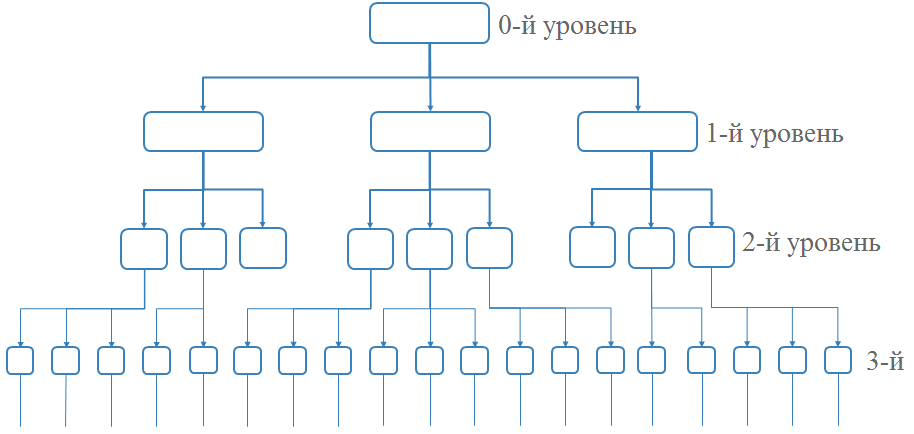
\includegraphics[width=0.9\textwidth]{2block.png}
	\caption{Блочно-иерархический подход к проектированию}
	\label{pic:2block}
\end{figure*}

В соответствии с блочно-иерархическим подходом в объекте проектирования может быть выделен ряд иерархических уровней (рис.~\ref{pic:2block}). На верхнем уровне подлежащий проектированию сложный объект состоит из ряда менее сложных элементов (например, для ОЭП -- приемная система, электронный блок обработки сигналов с выхода приемника излучения). Указанные элементы на более низком иерархическом уровне, в свою очередь, являются системами элементов менее сложной структуры (например, в приемную оптическую систему могут входить объектив, компенсатор, анализатор изображения, сканирующий блок). 

Далее подобное разделение на элементы может продолжаться до некоторого уровня, на котором дальнейшее разделение становится уже невозможным. Элементы, полученные на этом уровне, по отношению к объекту проектирования являются базовыми. Применительно к ОЭП такими базовыми элементами будут детали (оптические, механические) и различные комплектующие изделия (электро- и радиоэлементы, подшипники, электродвигатели).

Иерархия составных частей ОЭП при блочно-иерархическом подходе:
\begin{enumerate}
	\item Приборное устройство (или его конструируемая часть).
	\item Функциональная единица.
	\item Сборочная единица --- изделие, составные части которого подлежат соединению между собой сборочными операциями.
	\item Детали --- изделие, изготовленное из однородного (по наименованию и марке) материала без применения сборочных операций. (Или неделимые однородные тела, состоящие из элементов формы (геометрических поверхностей тел) и материала).
\end{enumerate}

Общий процесс проектирования при таком подходе представляется в виде движения по рассматриваемому дереву, при котором выполняются элементарные проектные операции на каждом уровне и на каждой ветви, т.е. структура проектирования также является блочно-иерархической, причем на каждом уровне и ветви процесс проектирования имеет дело с небольшим количеством элементов, рассматриваемых как целые, благодаря чему этот процесс достаточно несложен и вполне реализуем при нормальных ресурсах. Весь процесс проектирования, сплетающийся в виде блочно-иерархической структуры таких элементарных процессов, также теперь становится вполне реализуемым.

Такая структура позволяет осуществлять общий процесс проектирования, используя различные направления движения по блочно-иерархическому дереву. В зависимости от направления движения различают нисходящее, восходящее и смешанное проектирование.

\newthought{Нисходящее проектирование}\marginnote{\allcaps{НИСХОДЯЩЕЕ\break ПРОЕКТИРОВАНИЕ}}, как следует из его названия, начинается с верхнего уровня, где прибор рассматривается как целое, затем проектируется его структура первого уровня, затем второго. Результатом проектирования на данном уровне является техническое задание для проектирования на следующем, более низком уровне.

Нисходящее проектирование всегда гарантирует выполнение требований технического задания на каждом уровне и поэтому должно бы считаться наиболее рациональным, но на каком-то уровне процесс проектирования может остановиться из-за того, что при существующих физических, технических, технологических или экономических ограничениях решение обратной задачи и соблюдение технического задания данного уровня становится невозможным. 

В этом случае приходится возвращаться на предыдущий уровень или даже выше, искать там другое решение своей обратной задачи, а затем опять пробовать вернуться на тот уровень, на котором процесс остановился, но с уже другим техническим заданием. 

Таким образом, блочно-иерархическая структура, позволяя в принципе реализовать процесс проектирования, делает неизбежным его итерационный характер, заключающийся в возврате к повторению проектирования на предыдущих уровнях с измененными условиями.

\newthought{Восходящее проектирование}\marginnote{\allcaps{ВОСХОДЯЩЕЕ\break ПРОЕКТИРОВАНИЕ}} выполняется в обратном порядке; при этом происходит как бы сборка отдельных узлов, а затем сборка всего прибора. 

Восходящее проектирование, как нетрудно увидеть, обычно гарантирует реализуемость проекта на любом уровне, но отнюдь не гарантирует соблюдения всех требований технического задания, поэтому процесс может остановится на каком-либо уровне из-за несоблюдения требований технического задания высшего уровня. При этом необходим возврат на предыдущие низшие уровни с попыткой <<собрать>> структуру данного уровня из других элементов. 
Таким образом и восходящее проектирование также неизбежно имеет итерационный характер.


\newthought{При смешанном проектировании }\marginnote{\allcaps{СМЕШАННОЕ\break ПРОЕКТИРОВАНИЕ}} по части ветвей мы имеем нисходящий процесс, а по части~-- восходящий, которые в определенных точках встречаются. Итерационный характер такого проектирования также очевиден.

Из рассмотренных процессов предпочтительным является все-таки нисходящее проектирование. На практике, особенно для сложных приборов, процесс проектирования носит обычно смешанный характер с преобладанием нисходящих потоков, а восходящее проектирование применяется к тем частям приборов, которые собираются из стандартных, хорошо отработанных деталей, элементов и узлов.

Из рассмотренного становится ясен также эвристический характер проектирования, т.е. невозможность его полной алгоритмизации, автоматизации, поскольку ввиду сложности процесса и невозможности заранее определить полностью его ход необходимо принимать решения на основании опыта, интуиции, с привлечением творческих способностей разработчика, т.е. на базе так называемого алгоритма принятия решения. 

Все этапы проектирования выполняются на основе ТЗ. В случае, когда проектирование объекта проводится по сформулированным на более высоком иерархическом уровне ТЗ, оно носит название внутреннего. Внешнее проектирование предполагает разработку ТЗ на систему высшего иерархического уровня. При внешнем проектировании необходим правильный учет современного состояния техники, возможностей технологии, перспектив их развития, экономических факторов.

\section{Аспекты проектирования}
Любое техническое решение обладает положительным и отрицательным эффектом. 

Применение САПР качественно улучшает процесс проектирования. 
Использование САПР позволяет:
\begin{itemize}
	\item проанализировать большое число различных схемных и конструктивных решений за короткий интервал времени;
	\item использовать более точные математические методы для расчёта и проектирования ОЭП;
	\item создавать конструкции, оптимально отвечающие предъявляемым к ним техническим требованиям;
	\item повышать качество конструкторской и технологической документации создаваемых ОЭП;
	\item проводить численные эксперименты, которые могут с достаточной степенью точности имитировать натурные испытания.
\end{itemize}

Идеальное техническое устройство --- устройство, которое выполняет свои функции, но его нет.

Существует большое количество методов проектирования, в том числе и большая группа эвристических\marginnote{Эвристика --- область знаний, основанная на творческом, неосознанном мышлении человека}:
\begin{itemize}
	\item теория решения изобретательских задач (ТРИЗ);
	\item мозговой штурм;
	\item метод итераций;
	\item метод контрольных вопросов;
	\item функционально-стоимостной анализ.
\end{itemize}

\newthought{ТРИЗ}\marginnote{\allcaps{ТРИЗ}} разработана в СССР Г.С.~Альтшуллером в 1956~г. 

ТРИЗ\marginnote{http://www.altshuller.ru/} является своего рода попыткой формализовать процесс проектирования и решения изобретательских задач. 

ТРИЗ развивает иной, более творческий тип мышления.
В ТРИЗ при проектировании используются различные приёмы, позволяющие решить технические противоречия.

\newthought{Мозговой штурм}\marginnote{\allcaps{МОЗГОВОЙ ШТУРМ}}:
\begin{itemize}
	\item Постановка задачи.
	\item Генерация идей.
	\begin{itemize}
		\item запрещена критика идей;
		\item приветствуются любые идеи;
		\item количество идей не ограничено.
	\end{itemize}
	\item Отбор идей.
\end{itemize}


\section{Основные требования, предъявляемые к ОЭП}

\newthought{Требования по внешним условиям и условиям эксплуатации}: к внешним условиям, оказывающим влияние на работу ОЭП, могут быть отнесены климатические факторы, механические воздействия, возникающие при транспортировании и эксплуатации, различные виды силовых полей, действие ионизирующего излучения.

В процессе эксплуатации различают два режима:
\begin{itemize}
	\item сохранение работоспособности ОЭП при воздействии дестабилизирующих факторов с экстремальными значениями (устойчивость);
	\item обеспечение работоспособности ОЭП в нормальных условиях после воздействия на неработающий прибор дестабилизирующих факторов с экстремальными значениями (прочность, стойкость).
\end{itemize}

Наиболее разнообразно влияние климатических факторов: температуры, влажности, давления окружающей среды, воздействия твердых и газообразных примесей, солнечного излучения, ветровой нагрузки, биофакторов.

\textsc{Температура}\marginnote{\allcaps{ТЕМПЕРАТУРА}} окружающей среды оказывает существенное влияние на работу приборов, так как при ее изменении практически все элементы и детали ОЭП меняют свои свойства. 
Диапазон температур, в котором приходится работать ОЭП, весьма широк. 
Даже в земных условиях возможны перепады температуры воздуха от $-80^{\circ}$C (в Антарктиде) до $+55^{\circ}$C (в тропических районах). 
При прямом воздействии Солнца температура нагретой поверхности может быть значительно выше. 
В отдельных случаях требуется обеспечить нормальную работу прибора в еще более жестких температурных условиях. 

Например, температура на поверхности Венеры достигает $300^{\circ}$С, а в условиях космического пространства при затенении от солнечного излучения близка к абсолютному нулю.

Большинство ОЭП эксплуатируется в нормальных температурных условиях. 
Для многих видов приборов, используемых на открытом воздухе, требуется обеспечить нормальную работу в интервале температур $-50\ldots+50^{\circ}$С. 
В отдельных случаях требуется обеспечение работы приборов в экстремальных условиях, указанных выше.

При недостаточном учете влияния перепадов температуры возможны ухудшение качества оптического изображения из-за термооптических аберраций и смещения плоскости изображения за счет температурных деформаций, появление расклеек в компонентах, разрушение оптических деталей вследствие разности показателей расширения оптических материалов и материалов оправ.

Тепловые воздействия на электронные элементы проявляются, в частности, в изменении параметров приемников излучения, номинальных значений параметров и характеристик электрорадиоэлементов, нарушении контактов и пробоях в изоляционных материалах.

В кинематических цепях при изменении температуры возможны ухудшение прочности материалов, повышение трения за счет изменения зазоров и вытекания или загустения смазочного материала. При неравномерном нагреве или охлаждении могут появляться деформации, приводящие к заклиниванию кинематических механизмов.

Весьма\marginnote{\allcaps{ВЛАГА}} серьезные последствия оказывает на приборы попадание \textsc{влаги}. 
Наличие влаги может привести к запотеванию оптических деталей, особенно в сочетании с резким изменением температуры. 
Пары воды, вступая в химическую реакцию с материалами, приводят к коррозии металлов, изменению физико-химических свойств специальных покрытий оптических деталей и изоляционных материалов. 
Под воздействием влаги ухудшаются контактные соединения за счет окисления контактов.

При проектировании предусматривают меры по защите приборов от воздействия влаги. Часто с этой целью приборы герметизируют, а внутренний объем осушают продувкой сухого очищенного воздуха. Могут применяться также специальные влагопоглотители.

\textsc{Давление}\marginnote{\allcaps{ДАВЛЕНИЕ}} окружающей среды оказывает заметное влияние на функционирование ОЭП. При понижении давления воздуха падает значение напряжения пробоя, что особенно важно помнить при использовании высоковольтных элементов. Кроме этого, существенно возрастает скорость испарения смазочного материала, что может привести к повышению трения и заклиниванию элементов кинематики прибора. В связи с уменьшением давления отвод теплоты за счет конвекционного переноса падает, в результате чего резко возрастает вероятность перегрева элементов прибора. Поэтому необходимо либо применять специальные материалы и элементы, рассчитанные на работу в условиях пониженного давления, либо осуществлять герметизацию прибора с созданием нормального рабочего давления внутри.

На\marginnote{\allcaps{ПЕСОК И ПЫЛЬ}} работу ОЭП оказывают влияние не только рассмотренные выше климатические факторы, но и содержащиеся в воздухе \textsc{песок и пыль}. Их механическое воздействие в сочетании с воздействием влаги и нагрева иногда приводит к значительному ухудшению характеристик приборов.

В сочетании с ветровым воздействием наличие в воздухе частиц песка и пыли приводит к абразивному разрушению полированных и окрашенных поверхностей. При этом вследствие матирующего эффекта возможен выход из строя оптических систем.

Для\marginnote{\allcaps{СОЛНЕЧНОЕ ИЗЛУЧЕНИЕ}} приборов, эксплуатируемых на открытом воздухе, необходимо учитывать \textsc{воздействие солнечного излучения}, приводящее к перегревам, нарушениям лакокрасочных покрытий, усилению коррозии при одновременном воздействии кислорода и влаги воздуха, быстрому старению резины, пластмасс и электрической изоляции.

При\marginnote{\allcaps{БИОФАКТОРЫ}} длительной эксплуатации и хранении приборов, а также при эксплуатации в тропических условиях следует учитывать \textsc{влияние биофакторов}, к которым относятся плесневые грибы, насекомые и грызуны. Развитие плесени ухудшает механические и электрические параметры приборов, а также пропускание оптических деталей. Борьба с влиянием этого фактора сводится к герметизации и осушке внутренних объемов приборов, применению стекол группы А, защите оптических деталей специальными покрытиями, использованию фунгицидов. Кроме того, могут быть использованы такие методы, как придание корпусам и наружным деталям простой формы без углублений, пазов, выступов, которые способствуют скоплению грязи и пыли и затрудняют чистку приборов.

Важное\marginnote{\allcaps{МЕХАНИЧЕСКИЕ\break ВОЗДЕЙСТВИЯ}} значение при конструировании ОЭП имеет учет \textsc{влияния механических воздействий}, к которым относятся вибрация, ударные воздействия, транспортировочные перегрузки. При этом следует иметь в виду, что наряду с внешними источниками воздействий на элементы прибора могут оказывать влияние вибрация и удары, обусловленные внутренними источниками, например несбалансированностью вращающихся частей, неточностью изготовления, зазорами, разрушениями соприкасающихся кинематических элементов.

В результате воздействий указанных факторов возможны разрушения отдельных элементов, деталей и паек, нарушение контактов реле, переключателей, потенциометров и коллекторов, повреждение изоляции с возникновением замыканий, самоотвинчивание резьбовых соединений, появление трещин, сколов в оптических и других хрупких деталях.

Механическая прочность конструкции обеспечивается применением соответствующих материалов, способов соединения деталей и может быть повышена за счет использования различных элементов жесткости: косынок, приливов, ребер.

Для предотвращения самоотвинчивания крепежных изделий либо применяют различные фиксаторы, либо устанавливают крепежные детали с использованием клеев, компаундов и герметиков. 

В случаях, когда указанные меры оказываются недостаточными, для защиты от механических воздействий используются демпферы и амортизаторы.

При\marginnote{\allcaps{ВОЗДЕЙСТВИЕ ПОЛЕЙ}} работе ОЭП подвергаются \textsc{воздействию различных полей}: электрического, магнитного, электромагнитного СВЧ, в результате чего могут возникать паразитные наводки, приводящие к ухудшению работы прибора. Источники полей могут находиться как вне, так и внутри прибора. Подавление наводок в большинстве случаев сводится к устранению или ослаблению паразитных связей между источником и приемником наводок путем экранирования и развязывания цепей.

Для защиты от электрических полей или подавления паразитной емкостной связи во всех диапазонах частот используют тонкие листы и пленки, а также проволочные сетки и решетки из материала с хорошей электрической проводимостью.

Для экранирования магнитных низкочастотных полей используют материалы с высокой магнитной проницаемостью (пермаллой, альсифер, технически чистое железо).

Для экранирования высокочастотных полей используют экраны из хорошо проводящих материалов (медь, латунь, алюминий). При действии полей СВЧ на основной материал экрана наносят слой серебра для повышения его электрической проводимости. 

Для защиты от наводок все электрические связи между блоками, по которым передаются измерительные сигналы, необходимо осуществлять экранированными проводами. Принципы расчета и конструирования защитных экранов изложены в соответствующей литературе.

Иногда\marginnote{\allcaps{ВОЗДЕЙСТВИЕ\break ИОНИЗИРУЮЩЕГО\break ИЗЛУЧЕНИЯ}} ОЭП используются в условиях \textsc{воздействия ионизирующего излучения} (на атомных электростанциях для дистанционного наблюдения, при космических исследованиях). 
Такие приборы должны отвечать требованиям радиационной стойкости. 
При воздействии ионизирующего излучения имеют место радиационные и поляризационные эффекты, приводящие к ухудшению оптических свойств материалов, нарушению работы полупроводниковых и электровакуумных приборов, изменению проводимости воздушных промежутков и диэлектрических материалов. 
При конструировании ОЭП, работающих в указанных условиях, прежде всего необходимо применять радиационно-стойкие материалы и элементы.

К ОЭП могут предъявляться также специфические требования, связанные с условиями эксплуатации. К их числу можно отнести, например, такие, которые вытекают из особенностей приборов, эксплуатируемых в состоянии невесомости, глубоко под водой, в шахтах. Кроме того, в некоторых ОЭП отдельные блоки могут работать в нормальных условиях, а остальные~-- в крайне неблагоприятных. Все эти особенности должны оговариваться при разработке ТЗ.

Таким образом, в современных условиях конструктору приходится иметь дело с широким кругом требований, которые находятся в тесном взаимодействии и часто противоречат друг другу, что приводит к многовариантности проектных решений.